\documentclass[11pt,a4paper]{article}
% ── Typography ────────────────────────────────────────────────────────────────
\usepackage[margin=2.5cm]{geometry}
\usepackage[utf8]{inputenc}
\usepackage[T1]{fontenc}
\usepackage{lmodern}
\usepackage{microtype}
% ── Colour, Graphics ─────────────────────────────────────────────────────────
\usepackage{xcolor}
\usepackage{tikz}
\usepackage{pgfplots}
\pgfplotsset{compat=1.18}
\usetikzlibrary{shapes.geometric, arrows.meta, positioning, fit, backgrounds,
                decorations.pathreplacing, calc, shadows.blur}
% ── Tables ───────────────────────────────────────────────────────────────────
\usepackage{booktabs}
\usepackage{array}
\usepackage{colortbl}
\usepackage{multirow}
% ── Document ─────────────────────────────────────────────────────────────────
\usepackage{listings}
\usepackage{hyperref}
\usepackage{enumitem}
\usepackage{fancyhdr}
\usepackage{amsmath}
\usepackage{amssymb}

% ── Colour palette ────────────────────────────────────────────────────────────
\definecolor{fpgablue}{RGB}{13,71,161}
\definecolor{fpgalight}{RGB}{187,222,251}
\definecolor{fpgamid}{RGB}{100,160,220}
\definecolor{hostgreen}{RGB}{27,94,32}
\definecolor{hostlight}{RGB}{200,230,201}
\definecolor{ibkrorange}{RGB}{200,80,0}
\definecolor{ibkrlight}{RGB}{255,224,178}
\definecolor{sigred}{RGB}{183,28,28}
\definecolor{codegray}{RGB}{248,248,248}
\definecolor{arrowgray}{RGB}{80,80,80}
\definecolor{sectionbg}{RGB}{232,240,254}
\definecolor{noteblue}{RGB}{227,242,253}
\definecolor{noteborder}{RGB}{100,160,220}

% ── TikZ styles ───────────────────────────────────────────────────────────────
\tikzset{
  block/.style={rectangle, rounded corners=4pt, minimum width=3cm,
    minimum height=1cm, text centered, draw, font=\small\bfseries,
    text width=2.8cm},
  fpgablock/.style={block, fill=fpgalight, draw=fpgablue, text=fpgablue},
  hostblock/.style={block, fill=hostlight, draw=hostgreen, text=hostgreen},
  ibkrblock/.style={block, fill=ibkrlight, draw=ibkrorange, text=ibkrorange},
  arrow/.style={-{Stealth[length=6pt]}, thick, color=arrowgray},
  fatarrow/.style={-{Stealth[length=8pt]}, line width=2pt, color=fpgablue},
  slowarrow/.style={-{Stealth[length=8pt]}, line width=2pt, color=ibkrorange},
  dashbox/.style={rectangle, rounded corners=6pt, dashed, inner sep=10pt},
  nsbox/.style={rectangle, rounded corners=3pt, fill=fpgalight,
    draw=fpgablue, font=\small\bfseries, inner sep=6pt, text=fpgablue},
  msbox/.style={rectangle, rounded corners=3pt, fill=ibkrlight,
    draw=ibkrorange, font=\small\bfseries, inner sep=6pt, text=ibkrorange},
}

% ── Page style ────────────────────────────────────────────────────────────────
\pagestyle{fancy}
\fancyhf{}
\rhead{\small\textcolor{fpgablue}{FPGA Tick-to-Trade}}
\lhead{\small Part 1: Foundation \& Architecture}
\cfoot{\small\thepage}
\renewcommand{\headrulewidth}{0.5pt}

\hypersetup{colorlinks=true, linkcolor=fpgablue, urlcolor=fpgablue,
            pdftitle={FPGA Tick-to-Trade Part 1}}

\lstset{
  backgroundcolor=\color{codegray}, basicstyle=\ttfamily\small,
  keywordstyle=\color{fpgablue}\bfseries, commentstyle=\color{gray}\itshape,
  stringstyle=\color{sigred}, breaklines=true, frame=single,
  rulecolor=\color{gray!40}, numbers=left, numberstyle=\tiny\color{gray},
  xleftmargin=1.5em, xrightmargin=0.5em,
}

% ── Note box helper ───────────────────────────────────────────────────────────
\newenvironment{notebox}{%
  \begin{center}
  \begin{tikzpicture}
  \node[rectangle, rounded corners=4pt, fill=noteblue, draw=noteborder,
        text width=13cm, inner sep=10pt, font=\small]
  \bgroup\begin{minipage}{13cm}}%
  {\end{minipage}\egroup;
  \end{tikzpicture}
  \end{center}}

% ─────────────────────────────────────────────────────────────────────────────
\begin{document}

% ── Title page ────────────────────────────────────────────────────────────────
\begin{titlepage}
\begin{tikzpicture}[remember picture, overlay]
  \fill[fpgablue] (current page.north west) rectangle
    ([yshift=-7cm]current page.north east);
  % subtle grid texture
  \foreach \x in {0,1,...,30} {
    \draw[white, opacity=0.04, very thin] ([xshift=\x*0.7cm]current page.north west)
      -- ([xshift=\x*0.7cm, yshift=-7cm]current page.north west);
  }
  \foreach \y in {0,1,...,10} {
    \draw[white, opacity=0.04, very thin] ([yshift=-\y*0.7cm]current page.north west)
      -- ([yshift=-\y*0.7cm]current page.north east);
  }
  \node[text=white, font=\fontsize{28}{34}\selectfont\bfseries, anchor=north west]
    at ([xshift=2.5cm, yshift=-2.0cm]current page.north west)
    {FPGA Tick-to-Trade};
  \node[text=white!85, font=\Large, anchor=north west]
    at ([xshift=2.5cm, yshift=-3.6cm]current page.north west)
    {Part 1 \textemdash\ Foundation \& Architecture};
  \node[text=white!60, font=\normalsize, anchor=north west]
    at ([xshift=2.5cm, yshift=-5.0cm]current page.north west)
    {Abhishek\ \ $\cdot$\ \ June 2026\ \ $\cdot$\ \ AWS F1 (UltraScale+ VU9P)};
  \node[text=white!50, font=\small\itshape, anchor=north west]
    at ([xshift=2.5cm, yshift=-6.0cm]current page.north west)
    {Target roles: FPGA Engineer / HFT Infrastructure \textemdash\ Citadel, DRW, Jump Trading, Optiver};
\end{tikzpicture}
\vspace*{8cm}
\tableofcontents
\end{titlepage}

% ─────────────────────────────────────────────────────────────────────────────
\section{Project Goal and Motivation}

The goal is to build a \textbf{portfolio-grade FPGA trading system} that demonstrates
the exact engineering skills HFT firms hire for:

\begin{itemize}[leftmargin=1.5em, itemsep=2pt]
  \item RTL design in SystemVerilog — not HLS, not C/C++ with Vivado HLS
  \item Binary protocol parsing in hardware (NASDAQ TotalView-ITCH 5.0)
  \item Pipelining, fixed-point arithmetic, and hardware latency measurement
  \item Rigorous verification: golden-model comparison, cocotb, QuestaSim
\end{itemize}

The project is targeted at \textbf{FPGA Engineer} and \textbf{HFT Infrastructure} roles
at firms like Citadel Securities, DRW, Jump Trading, and Optiver,
in the \$125k--\$350k compensation range.

% ─────────────────────────────────────────────────────────────────────────────
\section{Background: Why Latency Matters in HFT}

\subsection{The Speed Arms Race}

High-Frequency Trading is an engineering discipline first. A strategy that is
\emph{correct but slow} loses money. The profit window for many HFT strategies
is measured in microseconds: the edge disappears the moment another firm quotes
a better price. A firm that can react to a market event 10\,$\mu$s faster than
its competitors will systematically capture fills at better prices.

This creates a direct economic incentive to reduce \emph{every nanosecond}
of latency in the signal processing chain:

\begin{center}
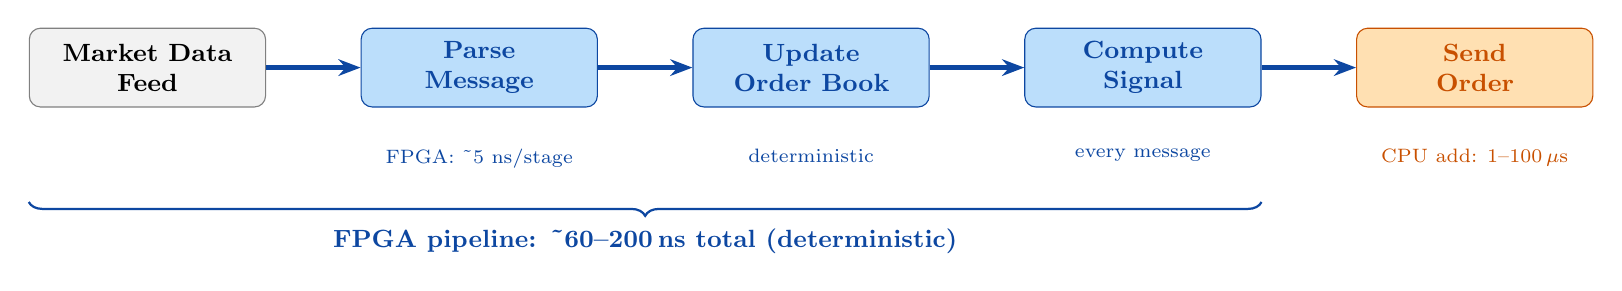
\begin{tikzpicture}[node distance=0.3cm and 1.5cm, font=\small]
  \node[block, fill=gray!10, draw=gray, text width=2.5cm] (feed)
    {Market Data\\Feed};
  \node[fpgablock, right=1.2cm of feed, text width=2.5cm] (parse)
    {Parse\\Message};
  \node[fpgablock, right=1.2cm of parse, text width=2.5cm] (book)
    {Update\\Order Book};
  \node[fpgablock, right=1.2cm of book, text width=2.5cm] (strat)
    {Compute\\Signal};
  \node[ibkrblock, right=1.2cm of strat, text width=2.5cm] (order)
    {Send\\Order};

  \draw[fatarrow] (feed) -- (parse);
  \draw[fatarrow] (parse) -- (book);
  \draw[fatarrow] (book) -- (strat);
  \draw[fatarrow] (strat) -- (order);

  \node[font=\scriptsize, below=0.4cm of parse, fpgablue] {FPGA: \textasciitilde{}5 ns/stage};
  \node[font=\scriptsize, below=0.4cm of book, fpgablue]  {deterministic};
  \node[font=\scriptsize, below=0.4cm of strat, fpgablue] {every message};
  \node[font=\scriptsize, below=0.4cm of order, ibkrorange] {CPU add: 1--100\,$\mu$s};

  % Total latency brace
  \draw[decorate, decoration={brace,amplitude=5pt,mirror}, thick, fpgablue]
    ([yshift=-1.2cm]feed.south west) -- ([yshift=-1.2cm]strat.south east)
    node[midway, below=6pt, font=\small\bfseries, fpgablue]
    {FPGA pipeline: \textasciitilde{}60--200\,ns total (deterministic)};
\end{tikzpicture}
\end{center}

\subsection{The p99 Tail Latency Problem}

CPU-based systems do not have a single latency — they have a \emph{distribution}.
The mean latency might be 2\,$\mu$s, but the 99th percentile (p99) can be 100$\times$
higher due to:

\begin{itemize}[itemsep=2pt]
  \item OS context switches and scheduler jitter
  \item CPU cache misses (L3 miss: \textasciitilde{}40\,ns; DRAM miss: \textasciitilde{}100\,ns)
  \item Hyper-threading contention
  \item Branch misprediction pipeline flushes
  \item Garbage collection (JVM/Python-based systems)
\end{itemize}

An FPGA has \textbf{no operating system, no cache hierarchy, no shared bus}.
Every message takes \emph{exactly} $N$ clock cycles. This is the key insight.

% ─────────────────────────────────────────────────────────────────────────────
\section{NASDAQ TotalView-ITCH 5.0 Protocol}

\subsection{What Is ITCH?}

NASDAQ TotalView-ITCH is a one-directional, UDP-multicast market data feed
published by NASDAQ. It carries the full limit order book for all NASDAQ-listed
equities in real time:

\begin{itemize}[itemsep=2pt]
  \item Every new order added to the book (\texttt{Add Order A})
  \item Every order partially or fully cancelled (\texttt{Order Cancel X}, \texttt{Order Delete D})
  \item Every order execution (\texttt{Order Executed E})
  \item Trade reports, cross trades, halt messages, and more
\end{itemize}

On a busy trading day, NASDAQ publishes \textasciitilde{}50 million messages.
Peak rates exceed 10 million messages/second. A CPU parsing these in software
with \textasciitilde{}200\,ns per message is already at 50\% utilisation just to keep up.

\subsection{Message Framing}

ITCH messages arrive in a \textbf{SoupBinTCP} or \textbf{MoldUDP64} frame.
Each message is prefixed with a 2-byte big-endian length field:

\begin{center}
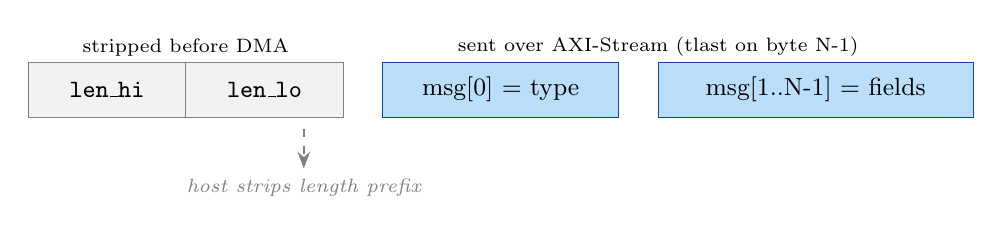
\begin{tikzpicture}[font=\small]
  \node[draw=gray, fill=gray!10, minimum width=2cm, minimum height=0.7cm,
        text centered] at (0,0) {\texttt{len\_hi}};
  \node[draw=gray, fill=gray!10, minimum width=2cm, minimum height=0.7cm,
        text centered] at (2,0) {\texttt{len\_lo}};
  \node[draw=fpgablue, fill=fpgalight, minimum width=3cm, minimum height=0.7cm,
        text centered] at (5,0) {msg[0] = type};
  \node[draw=fpgablue, fill=fpgalight, minimum width=4cm, minimum height=0.7cm,
        text centered] at (9,0) {msg[1..N-1] = fields};
  \node[font=\scriptsize, above=0.3cm] at (1,0) {stripped before DMA};
  \node[font=\scriptsize, above=0.3cm] at (7,0) {sent over AXI-Stream (tlast on byte N-1)};
  \draw[arrow, dashed, gray] (2.5, -0.5) -- (2.5, -1.0)
    node[below, font=\scriptsize\itshape]{host strips length prefix};
\end{tikzpicture}
\end{center}

The host software (\texttt{carve\_itch\_slice.py}) strips the 2-byte length prefix
and feeds raw message bytes to the FPGA via AXI-Stream DMA.
The parser sees only raw message bytes; \texttt{tlast} asserts on the final byte.

\subsection{Message Types Implemented}

Eight ITCH 5.0 message types are decoded. Add-with-MPID (F) and
Execute-with-Price (C) reuse the Add/Execute field layouts; Replace (U) carries
two order references; Trade (P) is an informational print (no book change).

\begin{center}
\begin{tabular}{c c l r l}
\toprule
\textbf{Type} & \textbf{ASCII} & \textbf{Name} & \textbf{Size} & \textbf{Key fields parsed} \\
\midrule
\texttt{0x41} & A & Add Order               & 36B & order\_ref, side, shares, price \\
\texttt{0x46} & F & Add Order with MPID     & 40B & as A (+ attribution, ignored) \\
\texttt{0x58} & X & Order Cancel            & 23B & order\_ref, cancelled\_shares \\
\texttt{0x44} & D & Order Delete            & 19B & order\_ref \\
\texttt{0x45} & E & Order Executed          & 31B & order\_ref, executed\_shares \\
\texttt{0x43} & C & Order Executed w/ Price & 36B & order\_ref, shares, exec price \\
\texttt{0x55} & U & Order Replace           & 35B & orig\_ref, new\_ref, shares, price \\
\texttt{0x50} & P & Trade (non-cross)       & 44B & order\_ref, side, shares, price \\
\bottomrule
\end{tabular}
\end{center}

% ─────────────────────────────────────────────────────────────────────────────
\section{The AXI-Stream Interface}

AXI4-Stream (AXIS) is the ARM AMBA standard for streaming data between IP
blocks on an FPGA. It is used throughout this design as the ``plumbing''
between the ITCH parser and the rest of the pipeline.

\subsection{Signal Handshake}

\begin{center}
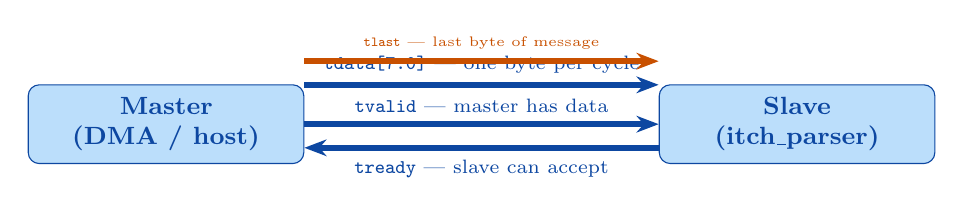
\begin{tikzpicture}[font=\small]
  \node[fpgablock, minimum width=3.5cm] (master) {Master\\(DMA / host)};
  \node[fpgablock, right=4.5cm of master, minimum width=3.5cm] (slave) {Slave\\(itch\_parser)};

  % Signals
  \draw[fatarrow] (master.east) -- node[above, font=\scriptsize]
    {\texttt{tvalid} — master has data} (slave.west);
  \draw[fatarrow] ([yshift=-0.3cm]slave.west) -- node[below, font=\scriptsize]
    {\texttt{tready} — slave can accept} ([yshift=-0.3cm]master.east);
  \draw[fatarrow] ([yshift=0.5cm]master.east) -- node[above, font=\scriptsize]
    {\texttt{tdata[7:0]} — one byte per cycle} ([yshift=0.5cm]slave.west);
  \draw[fatarrow, ibkrorange] ([yshift=0.8cm]master.east) -- node[above, font=\tiny]
    {\texttt{tlast} — last byte of message} ([yshift=0.8cm]slave.west);
\end{tikzpicture}
\end{center}

\begin{center}
\begin{tabular}{>{\ttfamily}l l}
\toprule
\textbf{Signal} & \textbf{Meaning} \\
\midrule
tvalid  & Master asserts: ``I have valid data this cycle'' \\
tready  & Slave asserts: ``I can accept data this cycle'' \\
tdata   & 8-bit data byte (one byte per clock in this design) \\
tlast   & Asserted on the \emph{last} byte of a message \\
\midrule
\multicolumn{2}{l}{Transfer occurs when \textbf{both} \texttt{tvalid} and \texttt{tready} are high} \\
\bottomrule
\end{tabular}
\end{center}

\noindent In this project, the parser always holds \texttt{tready = 1} (it can always
accept a byte). This simplifies the interface: a transfer happens every cycle
that \texttt{tvalid} is high. The parser counts bytes using \texttt{byte\_cnt}
and asserts \texttt{m\_valid} for one cycle when the last byte (\texttt{tlast}) arrives.

% ─────────────────────────────────────────────────────────────────────────────
\section{The Two-Path Architecture}

\subsection{Design Decision: Honest Two-Path Split}

Interactive Brokers is a retail brokerage — its API is rate-limited to
\textasciitilde{}50 messages/second and order round-trips take \textasciitilde{}30\,ms.
Claiming ``nanosecond trading through IBKR'' would immediately destroy
credibility with any HFT recruiter. The design therefore labels the two
paths honestly:

\vspace{0.8em}
\begin{center}
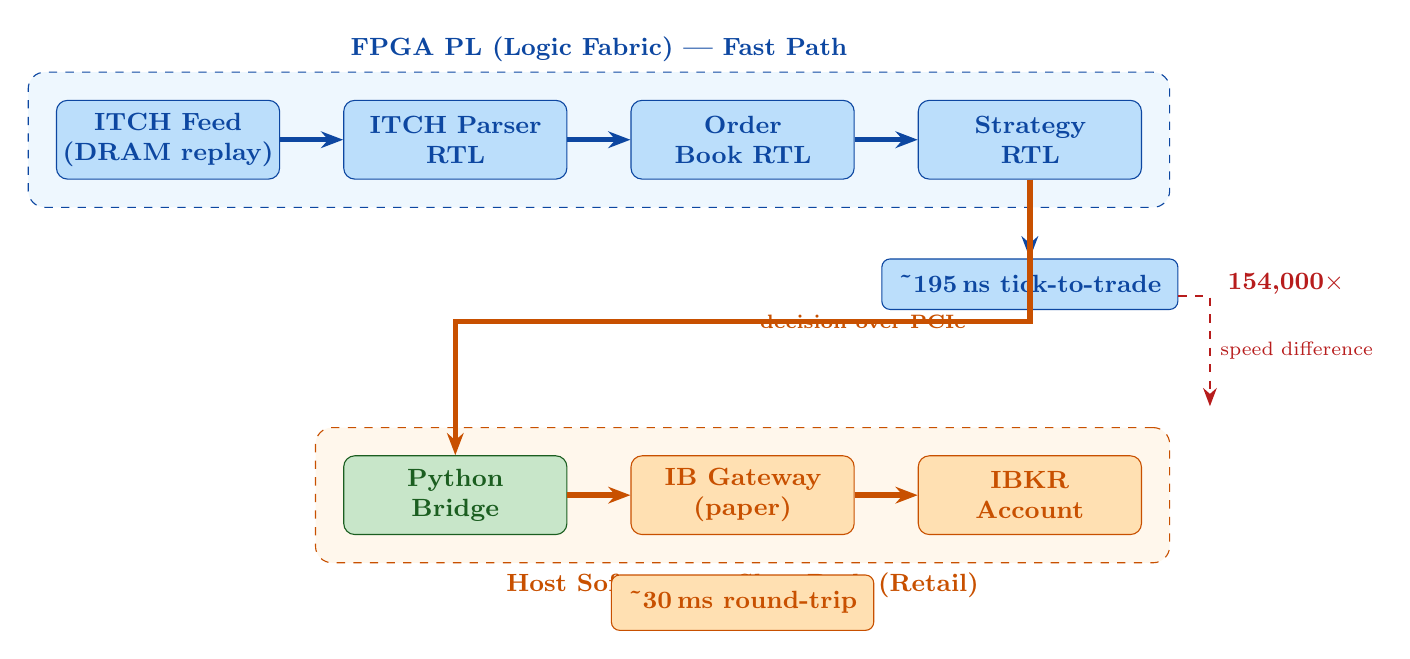
\begin{tikzpicture}[node distance=0.7cm and 1.2cm]

  %% ── FPGA fast path ──────────────────────────────────────────
  \node[fpgablock, minimum width=2.8cm, text width=2.6cm] (itch)
    {ITCH Feed\\(DRAM replay)};
  \node[fpgablock, right=0.8cm of itch, minimum width=2.8cm, text width=2.6cm] (parser)
    {ITCH Parser\\RTL};
  \node[fpgablock, right=0.8cm of parser, minimum width=2.8cm, text width=2.6cm] (book)
    {Order\\Book RTL};
  \node[fpgablock, right=0.8cm of book, minimum width=2.8cm, text width=2.6cm] (strat)
    {Strategy\\RTL};

  \begin{scope}[on background layer]
    \node[dashbox, fill=fpgalight!25, draw=fpgablue,
          fit=(itch)(strat), inner sep=10pt,
          label={[fpgablue, font=\bfseries\small]above:FPGA PL (Logic Fabric) --- Fast Path}] {};
  \end{scope}

  \draw[fatarrow] (itch) -- (parser);
  \draw[fatarrow] (parser) -- (book);
  \draw[fatarrow] (book) -- (strat);

  % Fast path result
  \node[nsbox, below=1.0cm of strat] (nslab)
    {\textasciitilde{}195\,ns tick-to-trade};
  \draw[fatarrow] (strat.south) -- (nslab.north);

  %% ── Connection between paths ────────────────────────────────
  \node[hostblock, below=3.5cm of parser, minimum width=2.8cm, text width=2.6cm]
    (bridge) {Python\\Bridge};
  \node[ibkrblock, right=0.8cm of bridge, minimum width=2.8cm, text width=2.6cm]
    (gw) {IB Gateway\\(paper)};
  \node[ibkrblock, right=0.8cm of gw, minimum width=2.8cm, text width=2.6cm]
    (acc) {IBKR\\Account};

  \begin{scope}[on background layer]
    \node[dashbox, fill=ibkrlight!25, draw=ibkrorange,
          fit=(bridge)(acc), inner sep=10pt,
          label={[ibkrorange, font=\bfseries\small]below:Host Software --- Slow Path (Retail)}] {};
  \end{scope}

  % PCIe DMA path from FPGA decision to host
  \draw[slowarrow] (strat.south) -- ++(0,-1.8) -|
    node[near start, right=2pt, font=\scriptsize\bfseries, ibkrorange]
    {decision over PCIe} (bridge.north);

  \draw[slowarrow] (bridge) -- (gw);
  \draw[slowarrow] (gw)     -- (acc);

  \node[msbox, below=0.5cm of gw] {\textasciitilde{}30\,ms round-trip};

  %% ── Comparison annotation ───────────────────────────────────
  \node[font=\bfseries\small, sigred, right=0.5cm of nslab]
    {154{,}000$\times$};
  \draw[-{Stealth}, sigred, thick, dashed]
    ([yshift=-0.15cm]nslab.east) -- ++(0.4,0) -- ++(0,-1.4)
    node[right, yshift=0.7cm, font=\scriptsize, sigred]{speed difference};

\end{tikzpicture}
\end{center}

\subsection{The Headline Comparison}

The \textbf{single most compelling artifact} of the project is this latency chart.
The log scale is necessary because the two values differ by six orders of magnitude.

\vspace{0.5em}
\begin{center}
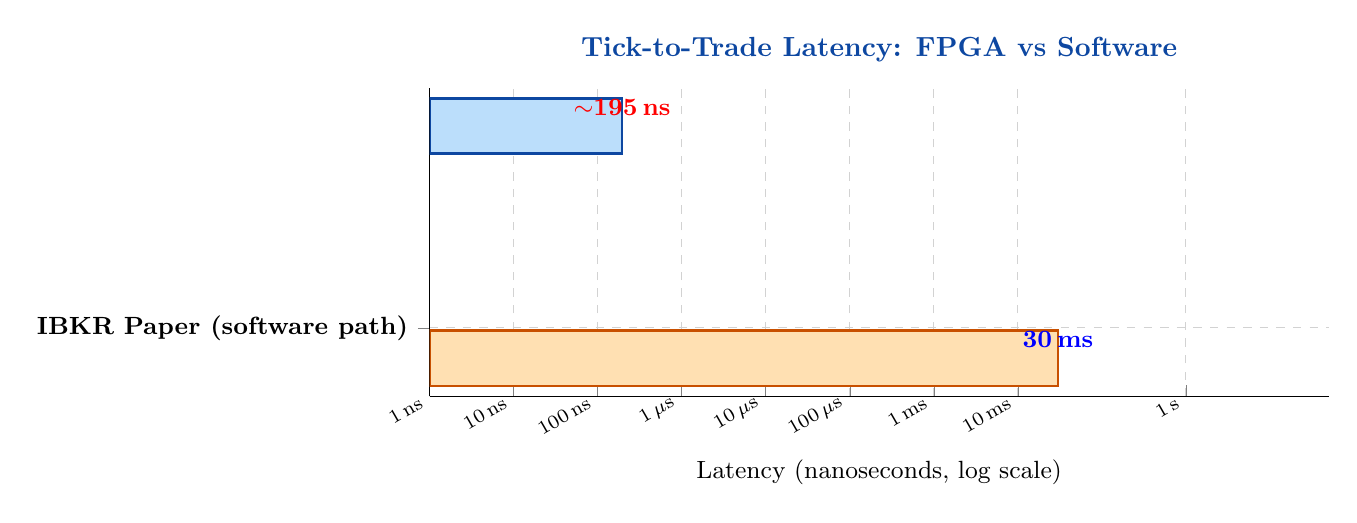
\begin{tikzpicture}
\begin{axis}[
  xbar, xmode=log,
  width=13cm, height=5.5cm,
  bar width=20pt,
  xlabel={Latency (nanoseconds, log scale)},
  xlabel style={font=\small},
  symbolic y coords={IBKR Paper (software path), FPGA Pipeline (hardware)},
  ytick=data,
  yticklabel style={font=\small\bfseries},
  xmin=1, xmax=5e10,
  xtick={1,10,100,1000,10000,100000,1000000,10000000,1000000000},
  xticklabels={1\,ns, 10\,ns, 100\,ns, 1\,$\mu$s, 10\,$\mu$s,
               100\,$\mu$s, 1\,ms, 10\,ms, 1\,s},
  xticklabel style={font=\scriptsize, rotate=30, anchor=east},
  nodes near coords,
  nodes near coords align={horizontal},
  every node near coord/.append style={font=\small\bfseries},
  point meta=explicit symbolic,
  axis x line*=bottom,
  axis y line*=left,
  grid=major, grid style={dashed, gray!35},
  title={\bfseries Tick-to-Trade Latency: FPGA vs Software},
  title style={font=\normalsize\bfseries, color=fpgablue},
  enlarge y limits=0.4,
]
\addplot+[fill=ibkrlight, draw=ibkrorange, line width=1pt]
  coordinates {(30000000,{IBKR Paper (software path)}) [30\,ms]};
\addplot+[fill=fpgalight, draw=fpgablue, line width=1pt]
  coordinates {(195,{FPGA Pipeline (hardware)}) [$\sim$195\,ns]};
\end{axis}
\end{tikzpicture}
\end{center}

% ─────────────────────────────────────────────────────────────────────────────
\section{Design Decisions}

Every key decision is documented with its rationale so interviewers can probe it.

\begin{center}
\small
\begin{tabular}{>{\bfseries}p{3.2cm} p{4.8cm} p{5.0cm}}
\toprule
Decision & Choice Made & Reason \\
\midrule
Logic style & RTL (SystemVerilog) — not HLS &
  HFT JDs explicitly ask for RTL; interviewers write RTL on whiteboards;
  HLS output is opaque for debugging \\
\addlinespace
Arithmetic & Fixed-point integers, no IEEE~754 floats &
  ITCH prices are already integers ($\times$10{,}000);
  no rounding error; one DSP block per multiply \\
\addlinespace
Delivery & Phased — M1 in weeks, then deepen &
  A working artefact to post sooner; reduces risk of a months-long project
  with nothing to show \\
\addlinespace
Execution path & IBKR paper account &
  Real confirmations, zero financial risk;
  clearly labelled as the slow path \\
\addlinespace
Hardware platform & AWS F1 (UltraScale+ VU9P) &
  PL-connected 25G Ethernet; no board purchase;
  real bitstream on real silicon \\
\addlinespace
Simulator & QuestaSim 2021.2 (Premium) &
  Industry standard; supports SystemVerilog, SVA,
  functional coverage; already installed \\
\addlinespace
Testbench & cocotb (Python) &
  Reuse the same Python golden model for both
  simulation driving and reference comparison \\
\bottomrule
\end{tabular}
\end{center}

% ─────────────────────────────────────────────────────────────────────────────
\section{Full System Architecture}

The diagram below shows every component and how data flows from the raw ITCH
file to an order in a paper account.

\begin{center}
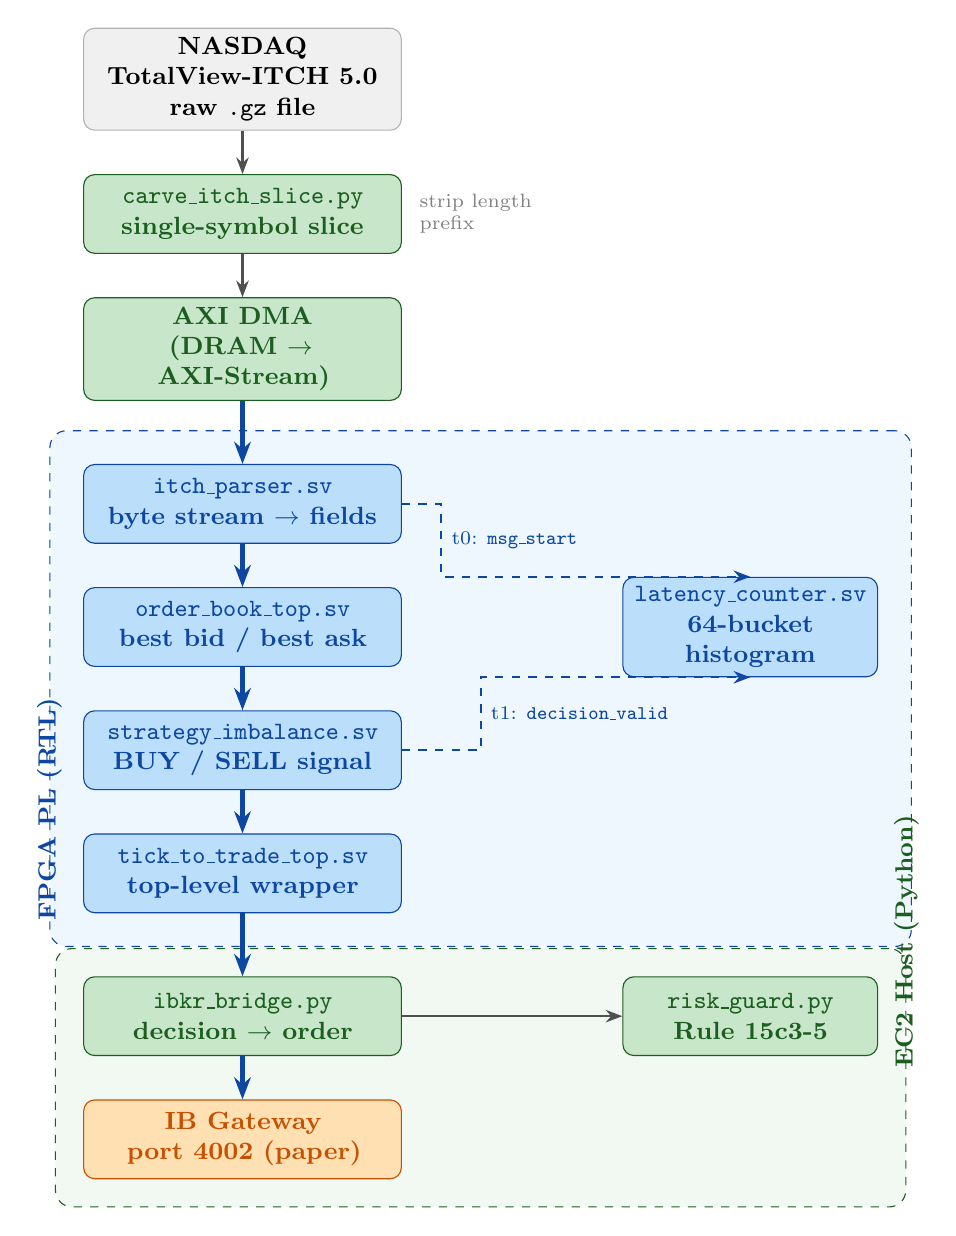
\begin{tikzpicture}[node distance=0.55cm and 0.5cm, font=\small]

  %% Data source
  \node[block, fill=gray!12, draw=gray!60, text width=3.8cm] (raw)
    {NASDAQ TotalView-ITCH 5.0\\raw \texttt{.gz} file};
  \node[hostblock, below=of raw, text width=3.8cm, minimum width=4cm]
    (carve) {\texttt{carve\_itch\_slice.py}\\single-symbol slice};
  \draw[arrow] (raw) -- (carve);
  \node[font=\scriptsize, right=0.1cm of carve, align=left, gray]
    {strip length\\prefix};

  %% DMA
  \node[hostblock, below=of carve, text width=3.8cm, minimum width=4cm]
    (dma) {AXI DMA\\(DRAM $\rightarrow$ AXI-Stream)};
  \draw[arrow] (carve) -- (dma);

  %% FPGA RTL pipeline
  \node[fpgablock, below=0.8cm of dma, minimum width=4cm, text width=3.8cm]
    (parser) {\texttt{itch\_parser.sv}\\byte stream $\rightarrow$ fields};
  \node[fpgablock, below=of parser, minimum width=4cm, text width=3.8cm]
    (book)   {\texttt{order\_book\_top.sv}\\best bid / best ask};
  \node[fpgablock, below=of book, minimum width=4cm, text width=3.8cm]
    (strat)  {\texttt{strategy\_imbalance.sv}\\BUY / SELL signal};
  \node[fpgablock, below=of strat, minimum width=4cm, text width=3.8cm]
    (top)    {\texttt{tick\_to\_trade\_top.sv}\\top-level wrapper};

  %% Latency counter (to the right)
  \node[fpgablock, right=2.8cm of book, minimum width=3.2cm, text width=3cm]
    (lat) {\texttt{latency\_counter.sv}\\64-bucket histogram};

  \begin{scope}[on background layer]
    \node[dashbox, fill=fpgalight!25, draw=fpgablue,
          fit=(parser)(top)(lat), inner sep=12pt,
          label={[fpgablue, font=\bfseries\small, rotate=90]left:FPGA PL (RTL)}] {};
  \end{scope}

  \draw[fatarrow] (dma)    -- (parser);
  \draw[fatarrow] (parser) -- (book);
  \draw[fatarrow] (book)   -- (strat);
  \draw[fatarrow] (strat)  -- (top);

  %% Latency taps
  \draw[arrow, dashed, fpgablue] (parser.east) -- ++(0.5,0)
    |- node[near start, right, font=\scriptsize, fpgablue]{t0: \texttt{msg\_start}} (lat.north);
  \draw[arrow, dashed, fpgablue] (strat.east)  -- ++(1.0,0)
    |- node[near start, right, font=\scriptsize, fpgablue]{t1: \texttt{decision\_valid}} (lat.south);

  %% Host software
  \node[hostblock, below=0.8cm of top, minimum width=4cm, text width=3.8cm]
    (bridge) {\texttt{ibkr\_bridge.py}\\decision $\rightarrow$ order};
  \node[hostblock, right=2.8cm of bridge, minimum width=3.2cm, text width=3cm]
    (risk)   {\texttt{risk\_guard.py}\\Rule 15c3-5};
  \node[ibkrblock, below=of bridge, minimum width=4cm, text width=3.8cm]
    (gw)     {IB Gateway\\port 4002 (paper)};

  \draw[fatarrow] (top)    -- (bridge);
  \draw[arrow]    (bridge.east) -- (risk.west);
  \draw[fatarrow] (bridge) -- (gw);

  \begin{scope}[on background layer]
    \node[dashbox, fill=hostlight!25, draw=hostgreen,
          fit=(bridge)(risk)(gw), inner sep=10pt,
          label={[hostgreen, font=\bfseries\small, rotate=90]right:EC2 Host (Python)}] {};
  \end{scope}

\end{tikzpicture}
\end{center}

% ─────────────────────────────────────────────────────────────────────────────
\section{Repository Layout}

\begin{center}
\small
\begin{tabular}{>{\ttfamily}l l}
\toprule
\textbf{Path} & \textbf{Contents} \\
\midrule
\texttt{rtl/}         & All synthesisable SystemVerilog modules \\
\quad\texttt{itch\_parser.sv}        & AXI-Stream slave, ITCH byte decoder, field shift registers \\
\quad\texttt{order\_book\_top.sv}    & M1: 256-entry direct-mapped order book (register file) \\
\quad\texttt{order\_book\_m2.sv}     & M2: multi-level book (top 4/side), RESCAN FSM, \texttt{msg\_ready} backpressure \\
\quad\texttt{strategy\_imbalance.sv} & Depth-weighted imbalance, spread guard, cooldown, scaled lots \\
\quad\texttt{latency\_counter.sv}    & Free-running counter + 64-bucket histogram, AXI-Lite readout \\
\quad\texttt{tick\_to\_trade\_top.sv}& Top wrapper: wires all RTL modules together \\
\midrule
\texttt{sim/}         & Simulation infrastructure \\
\quad\texttt{tb\_itch\_parser.py}    & cocotb testbench, 6 tests (all PASS) \\
\quad\texttt{Makefile}               & Questa + cocotb integration \\
\quad\texttt{synth\_itch.py}         & Synthetic ITCH message generator (no download needed) \\
\quad\texttt{golden/itch\_parser.py} & Python reference decoder \\
\quad\texttt{golden/order\_book.py}  & Python reference order book \\
\midrule
\texttt{host/}        & EC2 host software \\
\quad\texttt{ibkr\_bridge.py}        & Routes FPGA decisions to IBKR via \texttt{ib\_async} \\
\quad\texttt{risk\_guard.py}         & Pre-trade risk: size, fat-finger, rate, position, kill-switch \\
\midrule
\texttt{data/}        & Market data tooling \\
\quad\texttt{carve\_itch\_slice.py}  & Extracts single-symbol slice from ITCH \texttt{.gz} \\
\midrule
\texttt{docs/}        & This documentation (LaTeX + TikZ $\rightarrow$ PDF) \\
\bottomrule
\end{tabular}
\end{center}

% ─────────────────────────────────────────────────────────────────────────────
\section{Toolchain and Cost}

\begin{center}
\begin{tikzpicture}[node distance=0.5cm and 0.9cm, font=\small]
  \node[fpgablock, minimum width=3.2cm, text width=3cm, minimum height=1.1cm]
    (questa) {QuestaSim 2021.2\\Primary Simulator\\{\scriptsize SVA + coverage}};
  \node[fpgablock, right=0.8cm of questa, minimum width=3.2cm, text width=3cm, minimum height=1.1cm]
    (vivado) {Vivado ML\\Synthesis \& P\&R\\{\scriptsize on AWS AMI}};
  \node[hostblock, right=0.8cm of vivado, minimum width=3.2cm, text width=3cm, minimum height=1.1cm]
    (cocotb) {cocotb 2.0.1\\Python testbenches\\{\scriptsize VPI interface}};
  \node[hostblock, below=0.7cm of questa, minimum width=3.2cm, text width=3cm, minimum height=1.1cm]
    (python) {Python 3.12\\Golden model +\\{\scriptsize ITCH generator}};
  \node[ibkrblock, below=0.7cm of vivado, minimum width=3.2cm, text width=3cm, minimum height=1.1cm]
    (f1)     {AWS F1\\f1.2xlarge\\{\scriptsize \$1.65/hr (hardware only)}};
  \node[block, fill=gray!10, draw=gray, below=0.7cm of cocotb,
        minimum width=3.2cm, text width=3cm, minimum height=1.1cm]
    (veril)  {Verilator\\Smoke tests\\{\scriptsize free, fast}};

  \draw[arrow] (cocotb.west) -- (questa.east)
    node[midway, above, font=\scriptsize]{VPI};
  \draw[arrow] (python.north) -- (questa.south)
    node[midway, left, font=\scriptsize]{drives};
  \draw[arrow] (vivado.south) -- (f1.north)
    node[midway, right, font=\scriptsize]{AFI bitstream};
\end{tikzpicture}
\end{center}

\begin{center}
\small
\begin{tabular}{l l r}
\toprule
\textbf{Activity} & \textbf{Where} & \textbf{Cost} \\
\midrule
RTL simulation (all iterations) & Local Ubuntu VM & Free \\
Synthesis sanity check          & AWS EC2 (FPGA Dev AMI) & \textasciitilde\$0.10/hr \\
AFI bitstream build (one-time)  & AWS EC2 (Vivado) & \textasciitilde\$2--3 total \\
Hardware test on real VU9P      & AWS F1 f1.2xlarge & \$1.65/hr \\
\bottomrule
\end{tabular}
\end{center}

\noindent\textbf{No local Vivado install required} — the AWS FPGA Developer AMI includes
Vivado 2022.2 pre-installed. This saves \textasciitilde{}25\,GB of disk space.

% ─────────────────────────────────────────────────────────────────────────────
\section{Why FPGAs Beat CPUs for This Task}

\subsection{The Pipeline Model vs the Von Neumann Model}

A CPU processes one instruction at a time through a shared pipeline.
Multiple operations on the same data (parse $\to$ update $\to$ compare) happen
sequentially; the CPU must fetch, decode, and execute each step.

An FPGA implements all operations as \textbf{concurrent hardware}, all running
simultaneously on every clock cycle:

\begin{center}
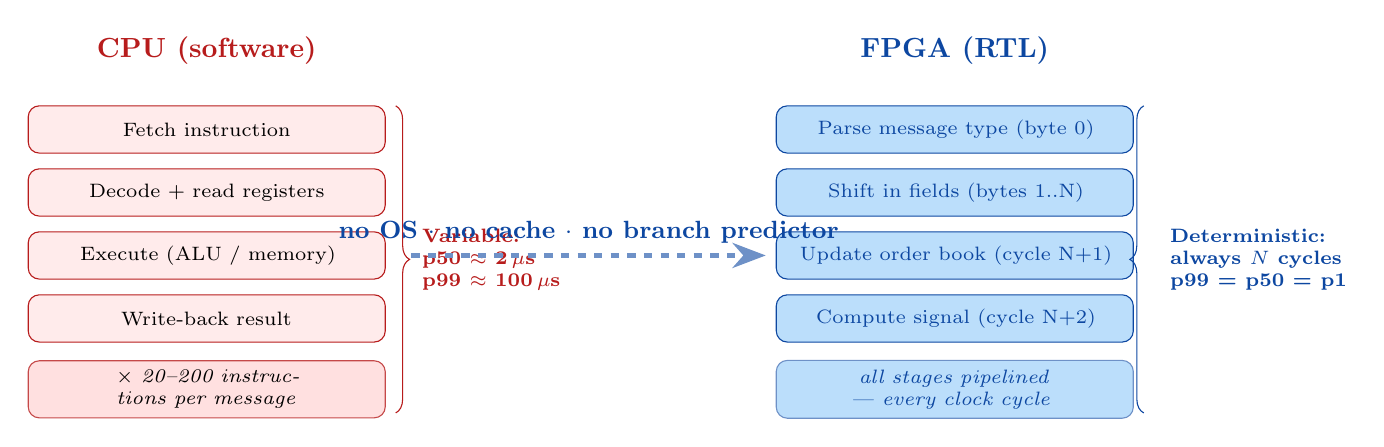
\begin{tikzpicture}[font=\small]

  %% CPU
  \node[font=\bfseries, sigred] at (0, 5.0) {CPU (software)};
  \node[block, fill=red!8, draw=sigred, minimum width=4.5cm, minimum height=0.6cm,
        font=\scriptsize, text width=4.3cm] at (0, 4.0)
    {Fetch instruction};
  \node[block, fill=red!8, draw=sigred, minimum width=4.5cm, minimum height=0.6cm,
        font=\scriptsize, text width=4.3cm] at (0, 3.2)
    {Decode + read registers};
  \node[block, fill=red!8, draw=sigred, minimum width=4.5cm, minimum height=0.6cm,
        font=\scriptsize, text width=4.3cm] at (0, 2.4)
    {Execute (ALU / memory)};
  \node[block, fill=red!8, draw=sigred, minimum width=4.5cm, minimum height=0.6cm,
        font=\scriptsize, text width=4.3cm] at (0, 1.6)
    {Write-back result};
  \node[block, fill=red!12, draw=sigred!80, minimum width=4.5cm, minimum height=0.6cm,
        font=\scriptsize\itshape, text width=4.3cm] at (0, 0.7)
    {$\times$ 20--200 instructions per message};

  \draw[decorate, decoration={brace,amplitude=5pt}, sigred]
    (2.4,4.3) -- (2.4,0.4) node[midway, right=6pt, font=\scriptsize\bfseries, sigred, align=left]
    {Variable:\\p50 $\approx$ 2\,$\mu$s\\p99 $\approx$ 100\,$\mu$s};

  %% FPGA
  \node[font=\bfseries, fpgablue] at (9.5, 5.0) {FPGA (RTL)};
  \node[fpgablock, minimum width=4.5cm, minimum height=0.6cm,
        font=\scriptsize, text width=4.3cm] at (9.5, 4.0)
    {Parse message type (byte 0)};
  \node[fpgablock, minimum width=4.5cm, minimum height=0.6cm,
        font=\scriptsize, text width=4.3cm] at (9.5, 3.2)
    {Shift in fields (bytes 1..N)};
  \node[fpgablock, minimum width=4.5cm, minimum height=0.6cm,
        font=\scriptsize, text width=4.3cm] at (9.5, 2.4)
    {Update order book (cycle N+1)};
  \node[fpgablock, minimum width=4.5cm, minimum height=0.6cm,
        font=\scriptsize, text width=4.3cm] at (9.5, 1.6)
    {Compute signal (cycle N+2)};
  \node[block, fill=fpgalight, draw=fpgablue!60, minimum width=4.5cm, minimum height=0.6cm,
        font=\scriptsize\itshape, text width=4.3cm, text=fpgablue] at (9.5, 0.7)
    {all stages pipelined — every clock cycle};

  \draw[decorate, decoration={brace,amplitude=5pt,mirror}, fpgablue]
    (11.9,4.3) -- (11.9,0.4) node[midway, right=6pt, font=\scriptsize\bfseries, fpgablue, align=left]
    {Deterministic:\\always $N$ cycles\\p99 = p50 = p1};

  %% Arrow
  \draw[-{Stealth}, line width=2pt, fpgablue!60, dashed]
    (2.6,2.4) -- (7.1,2.4)
    node[midway, above, font=\small\bfseries, fpgablue]
    {no OS $\cdot$ no cache $\cdot$ no branch predictor};

\end{tikzpicture}
\end{center}

\subsection{Fixed-Point Arithmetic --- No Division Required}

ITCH prices are 32-bit integers representing price\,$\times$\,10{,}000
(e.g., \$150.01 is stored as \texttt{1500100}). Division is \textbf{avoided entirely}
via the cross-multiplication identity:

\[
\frac{a}{b} > k \quad \Longleftrightarrow \quad a \cdot k_d > k \cdot b
\]

\noindent where $k = \frac{k_n}{k_d}$. For the imbalance signal with threshold
$k = 1.5 = \frac{15}{10}$:

\[
\text{bid\_size} \times 10 > 15 \times \text{ask\_size}
\]

\noindent Both sides require only one DSP multiply block each. The comparison
is a single combinational comparator. \textbf{No division, no floating-point unit,
no multi-cycle latency.}

\subsection{Determinism and FPGA Clock Discipline}

Every flip-flop in the FPGA changes state on exactly the same rising clock edge.
The critical path — the longest combinational path between two registers — determines
the maximum frequency. Vivado's timing engine reports the \emph{Worst Negative Slack}
(WNS). A positive WNS means timing is met; negative means the design must be
pipelined further or the clock slowed down.

At 200\,MHz (5\,ns period), and with a critical path of \textasciitilde{}4\,ns in the
strategy module, WNS $\approx$ +1\,ns. This leaves margin for process, voltage,
and temperature variation.

\end{document}
